%!TEX root = ../report.tex
\chapter{Hardware Architecture}
\label{ch:hardware}
This section describes the hardware architecture of \ProjectName{}. The description will be more high-level along with explanation about the hardware platform and the application interfaces between each components of the system. The rest of this chapter is organized as follows. First section, \autoref{sec:hardware-overview}, presents an overview of the hardware implemented in this system depicted in big schema. Decisions made in this system are detailed in \autoref{sec:hardware-decisions} with tables. Lastly, hardware description is described in \autoref{sec:hardware-description}.

\section{Hardware Overview}
\label{sec:hardware-overview}
The \ProjectName{} hardware components can be categorized into four main components: sensing part, data storing part, analytics part, and data presentation part. The data flow starts from wired and wireless sensors located across the Netherlands that collects information for monitoring. The process will end at data presentation and warning dispatch in the users' side. The overview of the hardware and its application interfaces are depicted in \autoref{fig:hardware-archi-schema} below.

% btw is it suppose to be the other way around? sensor monitoring -> analytics-> database ?
\begin{figure}[hb!]
\centering
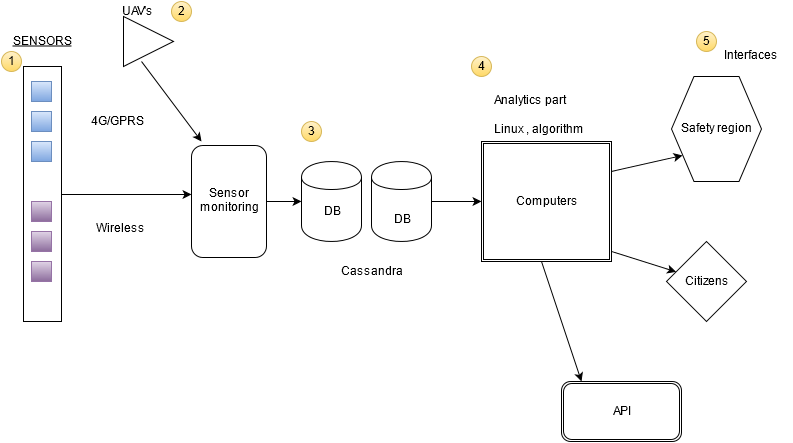
\includegraphics[scale=0.5]{images/HardwareArchitectureOverview.png}
\caption{Schematic overview of the hardware architecture of \ProjectName{}}
\label{fig:hardware-archi-schema}
\end{figure}

Here is an overview of the Hardware Architecture. Each number corresponds to a decision which will be detailed in the Hardware Design Decision part.

The \ProjectName{} will utilize wired and wireless sensor for monitoring water ways and dykes. Wired sensor will be placed in congested dykes and waterways where wired connection is possible. Wireless sensor will be planted in remote areas where wired connections are impossible or too costly. UAVs will fly to check reported faulty sensors. UAVs will also be used to take required pictures for further analytics or to examine some portion of the system which is hard or impossible for a personnel to access. Then all measurement will be forwarded to sensor monitoring part to be normalized before getting in to the analytics part.

The next part of the hardware is the cluster for carrying out analysis. This will be a collection of servers that is coordinated using clusters. This part also handles the logic for detecting faulty sensors, as the sensor monitoring parts contain no logic behind it.

We will use other cluster to store our important data. This cluster will run Cassandra database on top if it. This cluster will also have several interfaces to communicate with other instances, such as main analytics part, third party data gathering cluster, and API cluster.

The last part of the hardware architecture is third party data gathering cluster and API cluster. Third party data gathering cluster is responsible for collecting weather forecast and demographic information of the Netherlands. Meanwhile, API cluster is responsible for handling request from actors that will consume our practical information and for notifying safety region in case of imminent flood. Both of this cluster are merely collections of server computer that works together.

\section{Hardware Design Decisions}
\label{sec:hardware-decisions}
This section defines decisions made regarding the hardware selection. Tables will be used to make our justification in regard to hardware selection more crystal clear.

\begin{table}[h!]
\begin{tabular}{L{0.2\textwidth} L{0.6\textwidth}}
    \textbf{Name} 			& \textbf{Choice of the computer for data analyze} \\ \toprule
    \textbf{Decision} 		& \textbf{DEC-4}\\ \midrule
    \textbf{Status} 		& \textbf{Approved} \\ \midrule
    \textbf{Problem/Issue} 	& The system needs computer to analyze data from sensors, UAV's ,weather forecast. \\ \midrule
    \textbf{Decision} 		& IBM Supercomputer ...\\ \midrule
    \textbf{Alternatives} 	& \textit{BB}\\
    						& Other brand .\\
    						& \textit{BB}\\
    						& BBBB.\\
    						\midrule
    \textbf{Arguments} 		& IBM supercomputer uses Linux which is the oS we choosed. \\
    						& 	\begin{tabular}{l|lllllll|l}
							& 		\rot{Reliability} & \rot{Resilience} & \rot{Performance} & \rot{Security} & \rot{Scalability} & \rot{Cost} & \rot{\textbf{Score}} \\ \hline
							% 					
								\end{tabular} \\
    \\ \bottomrule
\end{tabular}

<<<<<<< HEAD

=======
IBM supercomputer uses Linux which is the oS we chose.
>>>>>>> 70d080df513435a0b6abf5648f080a2364ebaa4c
\caption{Decision -- Choice of computer}
\label{table:linux}
\end{table}

%Performance , Speed of calculation , Core ; lINUX

\begin{table}[h!]
\begin{tabular}{L{0.2\textwidth} L{0.6\textwidth}}
    \textbf{Name} 			& \textbf{Data representation - Interface with the third parties} \\ \toprule
    \textbf{Decision} 		& \textbf{DEC-4}\\ \midrule
    \textbf{Status} 		& \textbf{Approved} \\ \midrule
    \textbf{Problem/Issue} 	& The system needs to interact with the third parties. \\ \midrule
    \textbf{Decision} 		& Dashboard for the emergency services\\ Rack server \\ \midrule
    \textbf{Alternatives} 	& \textit{BB}\\
    						& DRAFT .\\
    						& \textit{BB}\\
    						& BBBB.\\
    						\midrule
    \textbf{Arguments} 		& \\

    \\ \bottomrule
\end{tabular}
\caption{Decision -- Interface with third parties}
\label{table:linux}
\end{table}



\begin{table}[h!]
\begin{tabular}{L{0.2\textwidth} L{0.6\textwidth}}
    \textbf{Name}           & \textbf{GeoBeads MEMS Sensor} \\ \toprule
    \textbf{Decision}       & \textbf{3}\\ \midrule
    \textbf{Status}         & \textbf{Approved} \\ \midrule
    \textbf{Problem/Issue}  & The system needs a reliable sensor system to measure condition of water ways and dykes. \\ \midrule
    \textbf{Decision}       & The system will implement GeoBeads MEMS Sensor in water ways and dykes.\\ \midrule
    \textbf{Alternatives}   & \textit{LiDAR}\\
                            & Remote sensing mechanism to measure condition of water ways.\\
                            \midrule
    \textbf{Arguments}      & \\
                            &   \begin{tabular}{l|lllllll|l}
                            &       \rot{Reliability} & \rot{Resilience} & \rot{Performance}& \rot{Interoperability} & \rot{Security} & \rot{Scalability} & \rot{Cost} & \rot{\textbf{Score}} \\ \hline
                            %                  rel res perf int sec sca cost
                                    GeoBeads   & 4 & 3 & 4 & 3 & 3 & 4 & 5 & 26\\ 
                                    LiDAR      & 2 & 4 & 3 & 3 & 4 & 4 & 2 & 22\\
                                \end{tabular} \\
    \\ \bottomrule
\end{tabular}
\caption{Decision -- Choice of Sensors}
\label{table:linux}
\end{table}

\section{Hardware Description}
\label{sec:hardware-description}
This section outlines describes description of the hardware implemented in this system. This section also supports decisions of hardware selection in previous section.

\subsection{Sensing Components}
\label{subsec:sensing-components}
Roughly 17.000 kilometers of dikes protect the Netherlands against flooding \cite{DMC}. 
The monitoring system consists of MEMS sensor modules (e.g. GeoBeads) with a claimed life time of 10 years, which are installed with conventional CPT push-in techniques. Three sensors are installed per cross-section and a cross-section is installed every 100 m. Each CPT push-in costs about \EUR{}200 per sensor (Feitsma,2002)\cite{TUDelftPHD}.%pp126

% Adds some picture here

\subsection{Database Cluster and Data Collection}
\label{subsec:database-data}
In the previous chapter, we decided to use Cassandra database as the database platform. However, Cassandra requires computers to run its environment. We decided to use clusters of computer to manage database system and to store our data. The cluster will also be accessible by other portions of our hardware, such as main analytics parts, third party data gathering part, and API part.

% Adds some picture here

\subsection{Analytics Components}
\label{subsec:analytics}

\subsection{Data Presentation}
\label{subsec:data-presentation}
